


\chapter{创造}

\section{问题}
\subsection{questions 1:1-5}
\begin{itemize}
\item What was created in the 1st day? 
\item Before the 1st day what were already there? 
\item In the 1st day, morning and evening, which appeared first?
\end{itemize}

\subsection{questions 1:6-13}
\begin{itemize}
\item What was created in the 2nd day?
\item What did the air separate?
\item What appeared in the 3rd day?
\end{itemize}

\subsection{questions 1:14-23}
\begin{itemize}
\item What did God created in the 4th day?
\item What did God created in the 5th day?
\end{itemize}


\subsection{questions 1:24-31}
\begin{itemize}
\item What did God created in the 6th day?
\item Human beings were created according to whose image?
\item Select which is human being’s food and which is animals food?
\begin{itemize}
\item A, All the trees whose fruits have seeds in them. 
\item B, All the green plants
\end{itemize}
\end{itemize}

\subsection{讨论}
\begin{itemize}
\item what did you learn about the characters of God?
\item Why human begins were created in the last day?
\end{itemize}

\newpage
\begin{figure}
\centering
     \begin{subfigure}[b]{0.43\textwidth}
         \centering
         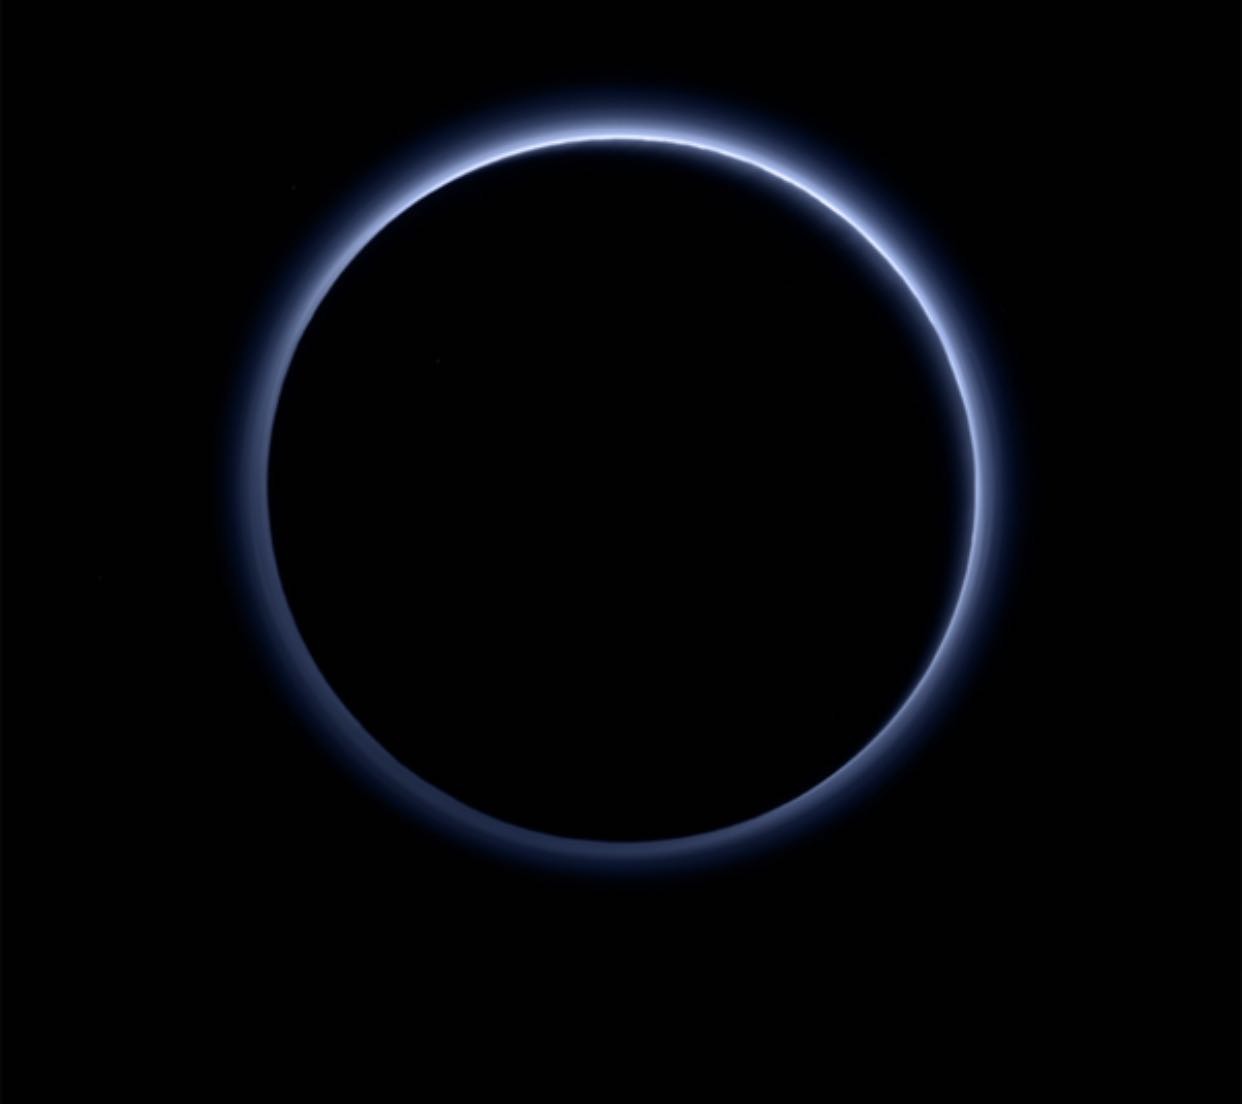
\includegraphics[scale=0.15, ]{ZongJie/bibleAdult/fig/beginning}
\caption{creation of the earth and heaven}
     \end{subfigure}
     \hfill
     \begin{subfigure}[b]{0.5\textwidth}
         \centering
         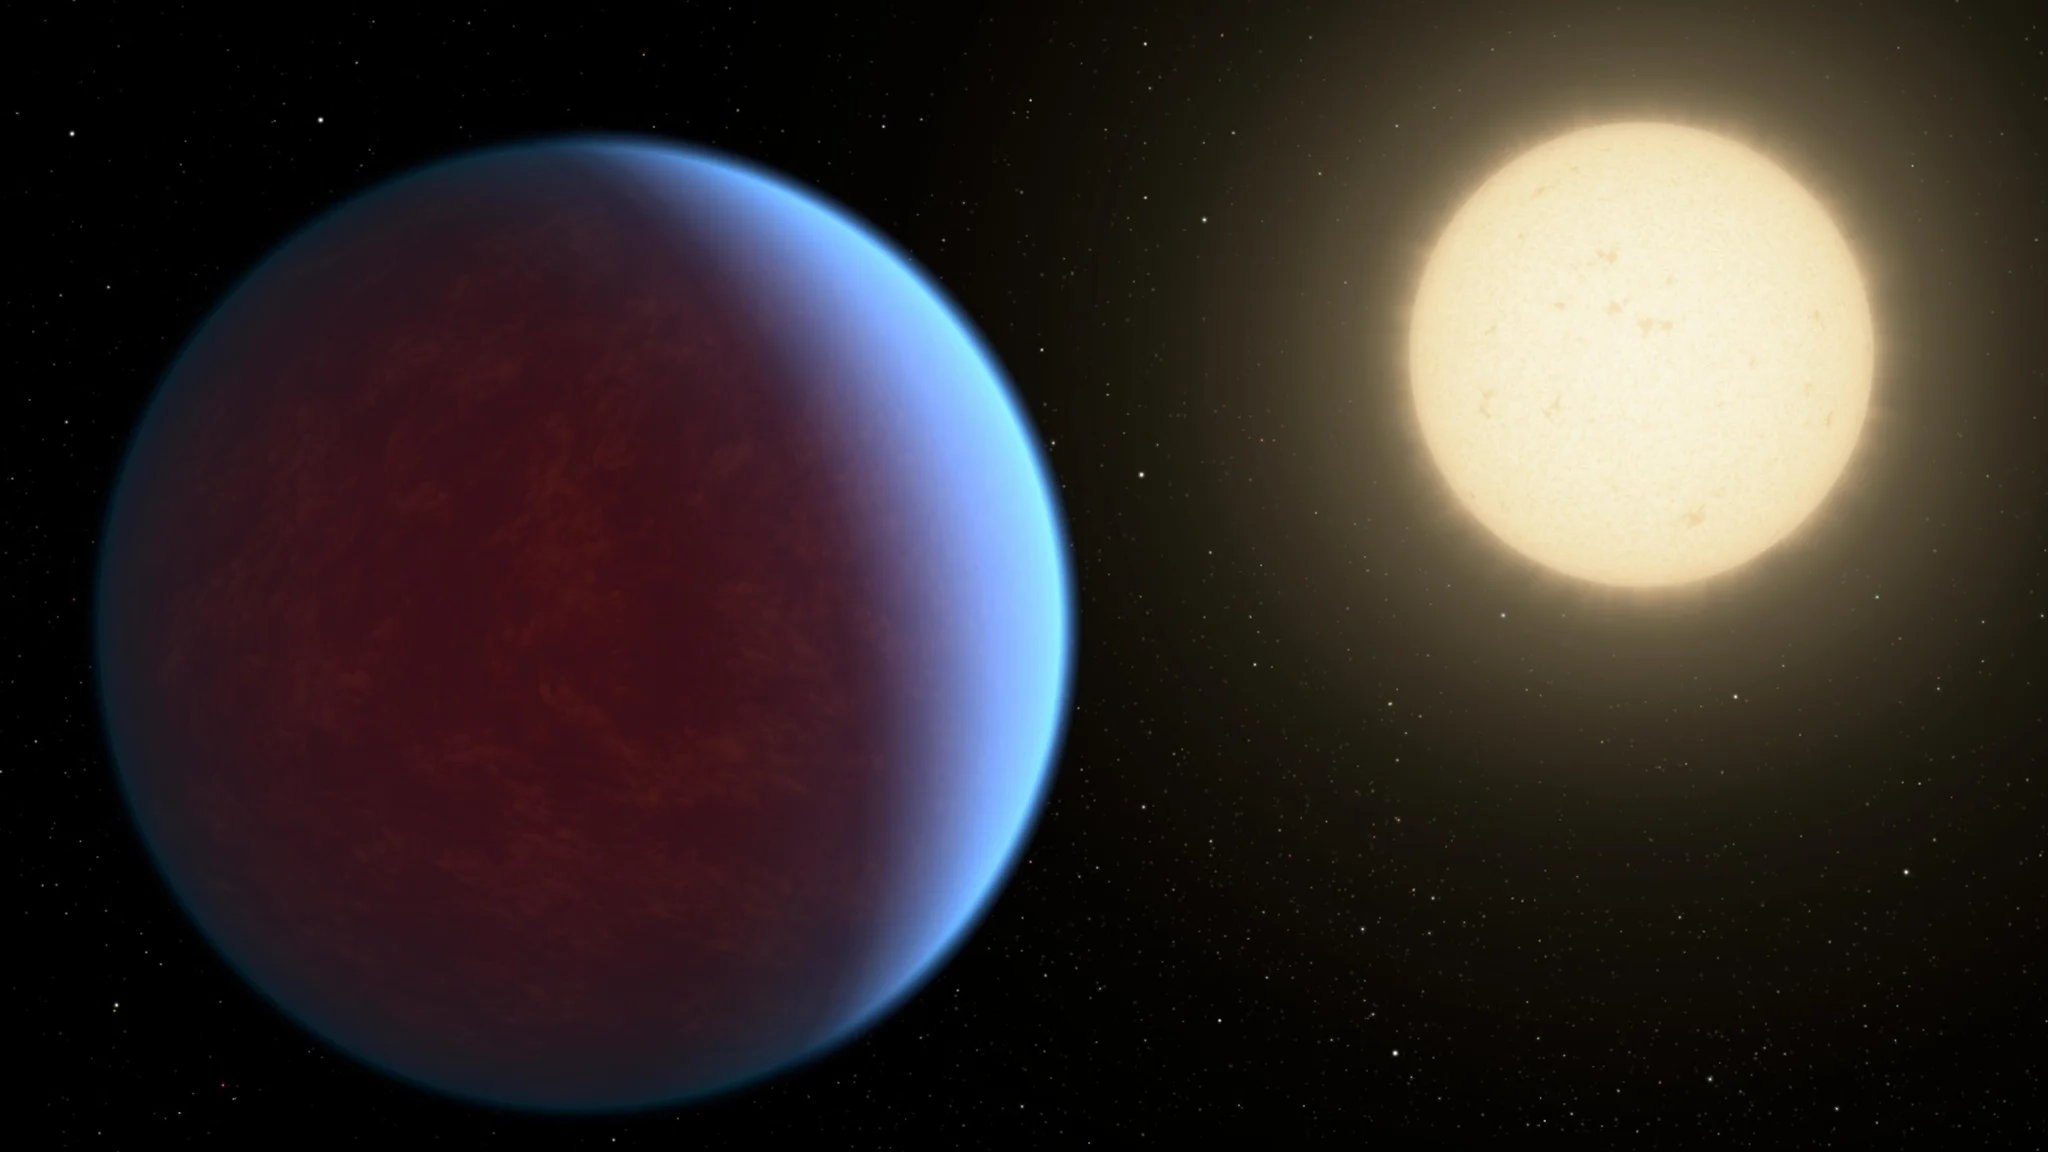
\includegraphics[scale=0.5, ]{ZongJie/bibleAdult/fig/day1}
\caption{creatioin of the light}
     \end{subfigure}
\end{figure}

\begin{figure}
\centering
     \begin{subfigure}[b]{0.3\textwidth}
         \centering
         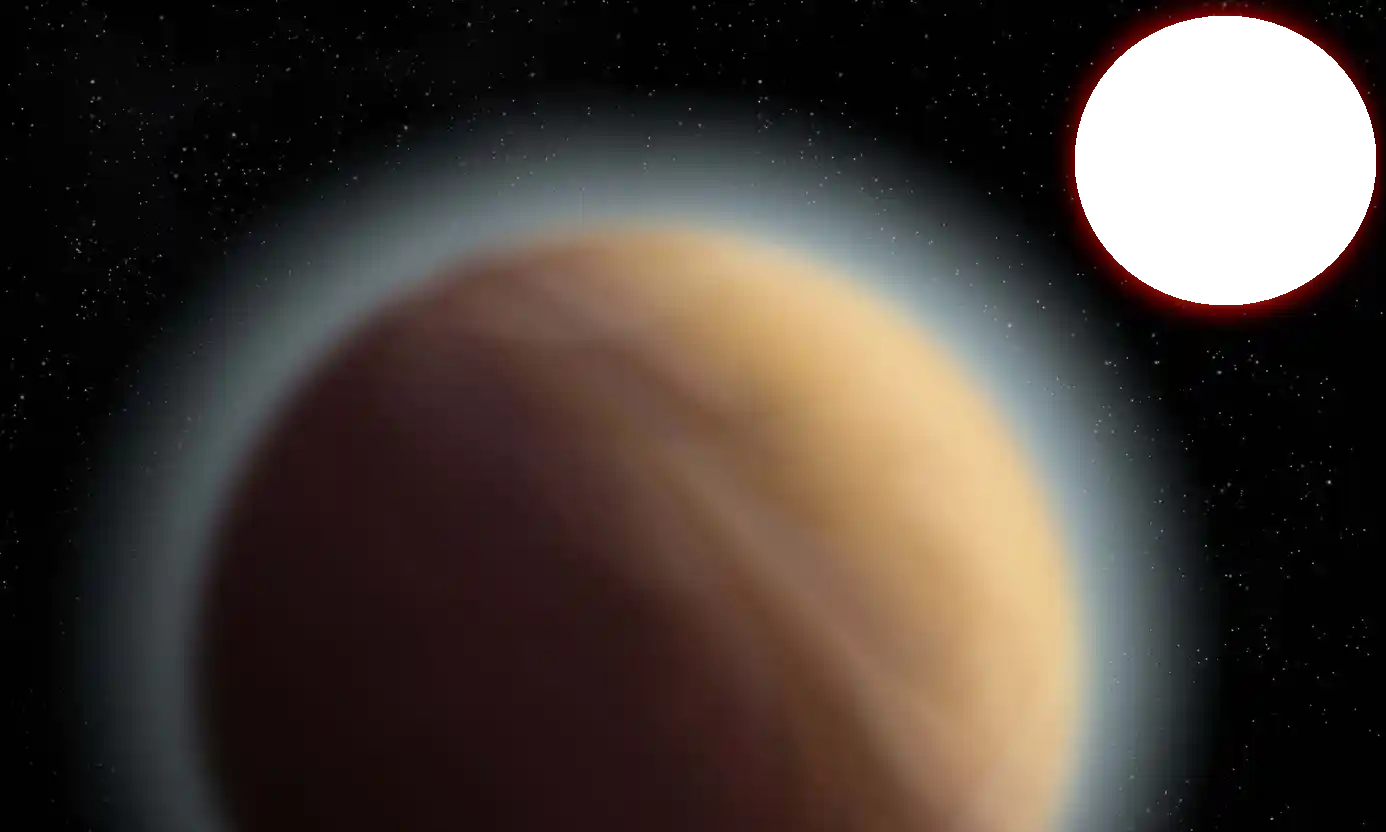
\includegraphics[scale=0.7, ]{ZongJie/bibleAdult/fig/day2}
\caption{creation of the air}
     \end{subfigure}
     \hfill
     \begin{subfigure}[b]{0.3\textwidth}
         \begin{center}
\hspace{-4.cm} 
\vspace{-.75cm}
   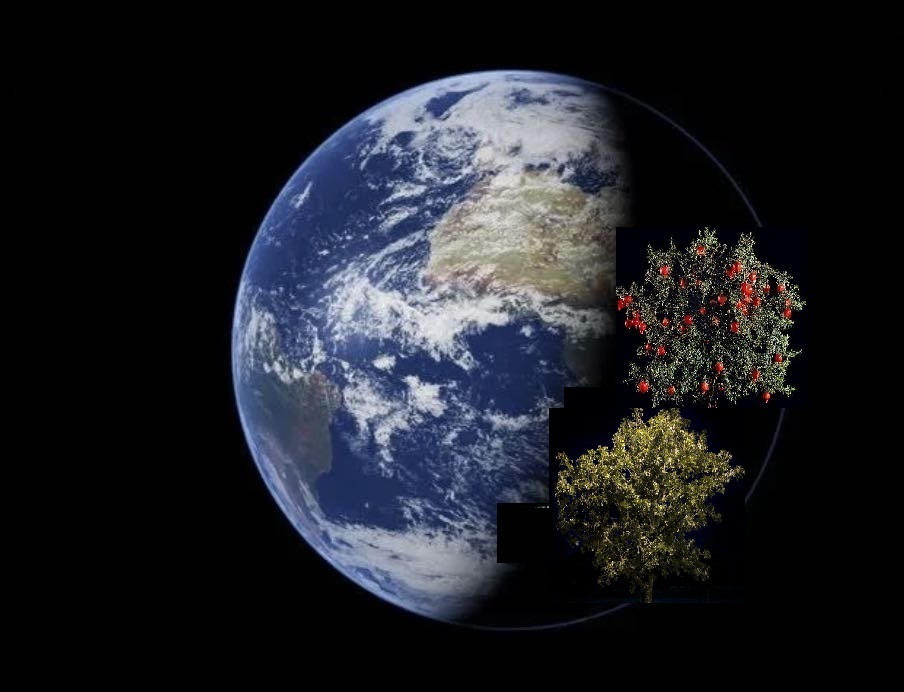
\includegraphics[scale=0.25]{ZongJie/bibleAdult/fig/2thday}
\end{center}
%\vspace{-.25cm}
\caption{creation of the land,sea and fruit trees}
     \end{subfigure}
\end{figure}

\begin{figure}
     \centering
     \begin{subfigure}[b]{0.3\textwidth}
         \centering
         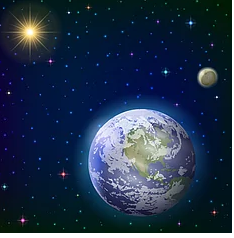
\includegraphics[width=\textwidth]{ZongJie/bibleAdult/fig/star1}
         \caption{creation of sun,moon and stars}
         \label{fig:y equals x}
     \end{subfigure}
     \hfill
     \begin{subfigure}[b]{0.3\textwidth}
         \centering
         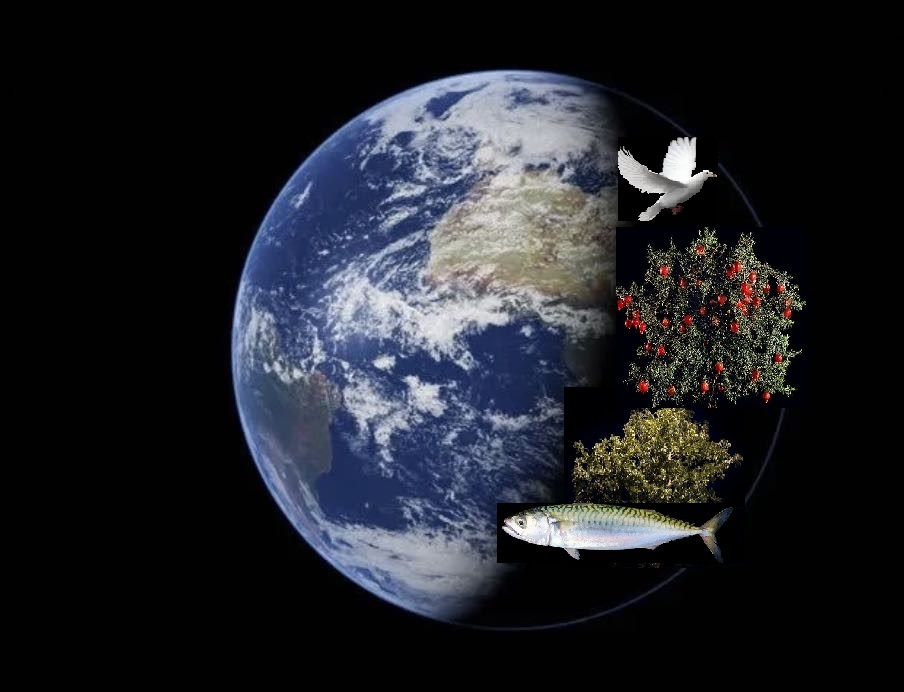
\includegraphics[width=\textwidth]{ZongJie/bibleAdult/fig/2ndday}
         \caption{creation of fish and bird}
         \label{fig:three sin x}
     \end{subfigure}
     \hfill
     \begin{subfigure}[b]{0.3\textwidth}
         \centering
         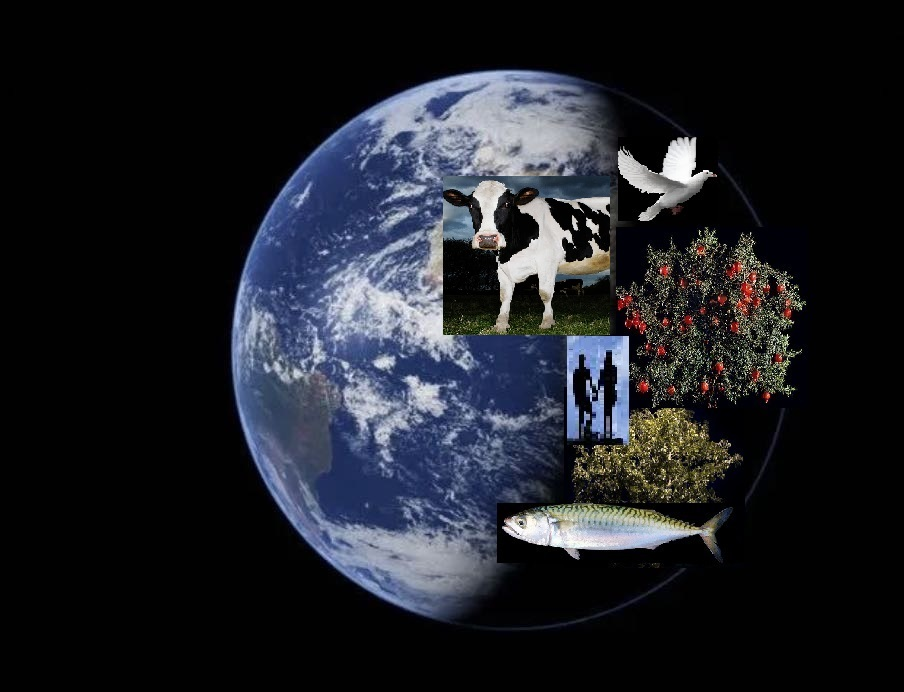
\includegraphics[width=\textwidth]{ZongJie/bibleAdult/fig/6day2}
         \caption{creation of man and woman}
         \label{fig:five over x}
     \end{subfigure}
      %  \caption{Three simple graphs}
     %   \label{fig:three graphs}
\end{figure}






\newpage
\begin{figure}
\centering
     \begin{subfigure}[b]{0.43\textwidth}
         \centering
  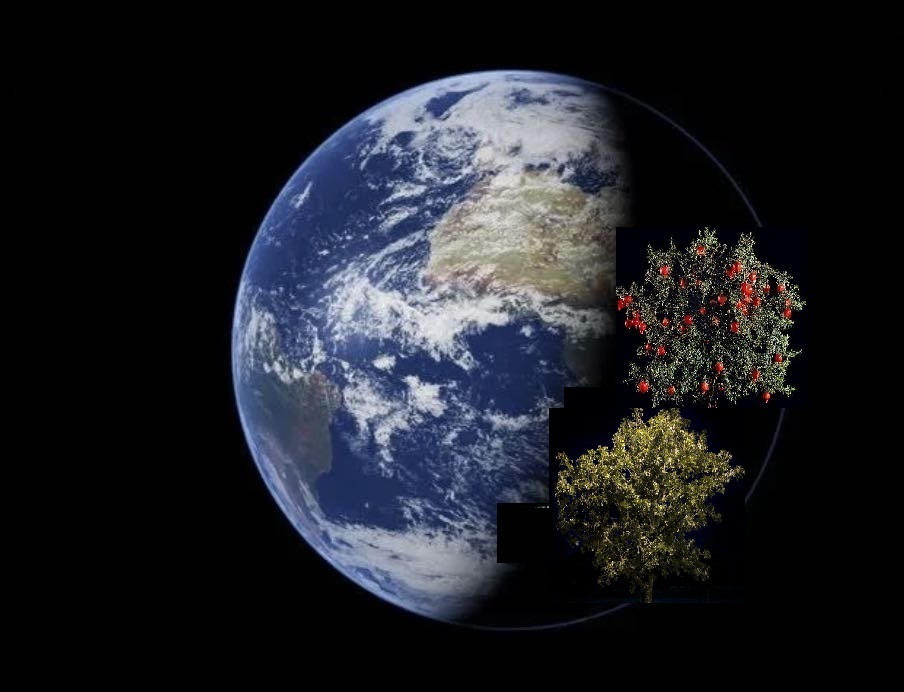
\includegraphics[scale=0.28]{ZongJie/bibleAdult/fig/2thday}       
%\caption{creation of the earth and heaven}
     \end{subfigure}
     \hfill
     \begin{subfigure}[b]{0.43\textwidth}
         \centering
 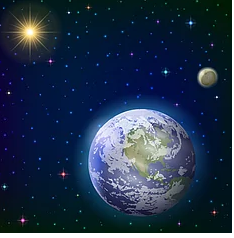
\includegraphics[width=\textwidth]{ZongJie/bibleAdult/fig/star1}
     \end{subfigure}
\end{figure}

\begin{figure}
\centering
     \begin{subfigure}[b]{0.3\textwidth}
         \centering
         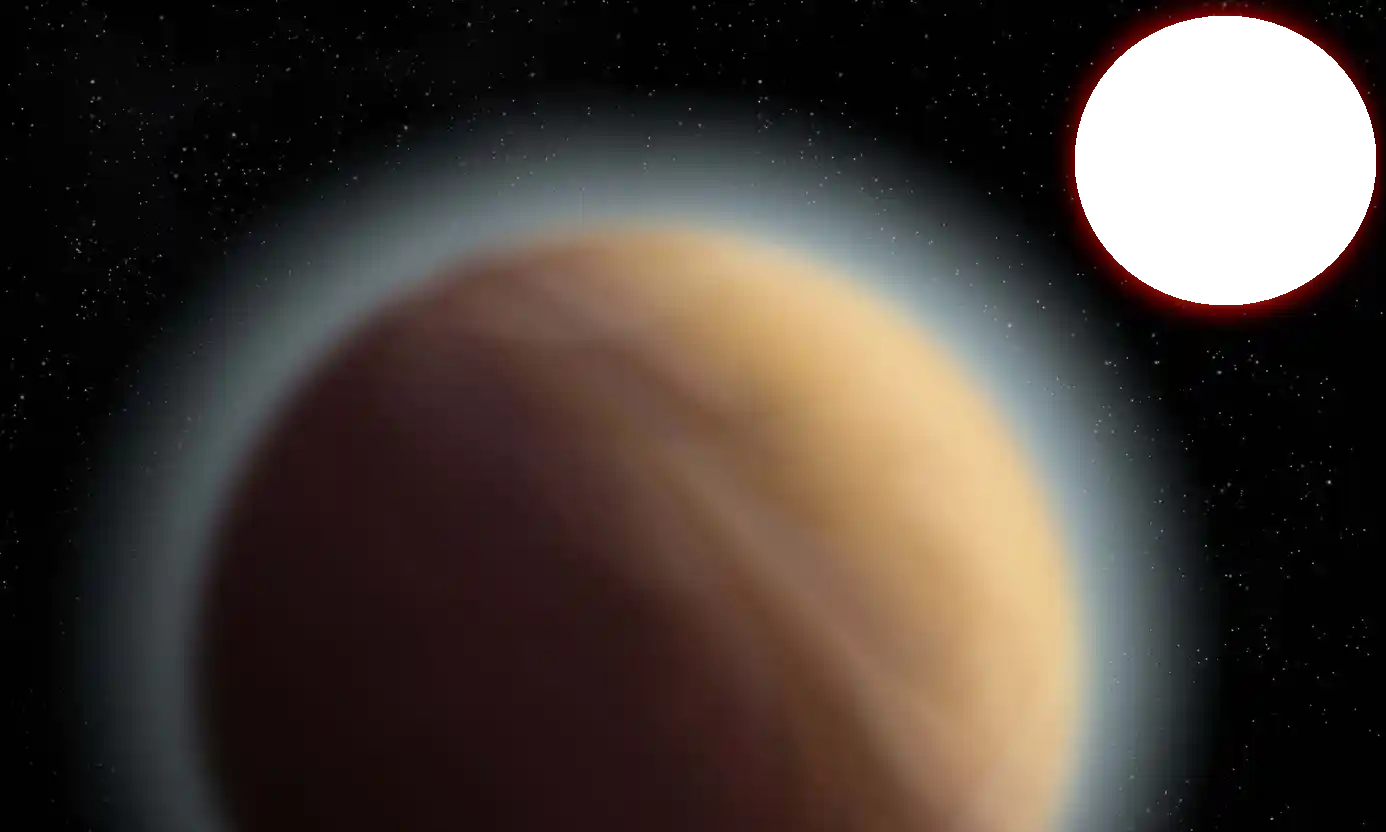
\includegraphics[scale=0.61, ]{ZongJie/bibleAdult/fig/day2}
%\caption{creation of the air}
     \end{subfigure}
     \hfill
     \begin{subfigure}[b]{0.4\textwidth}
         \begin{center}
\hspace{-2.5cm} \vspace{-.65cm}
 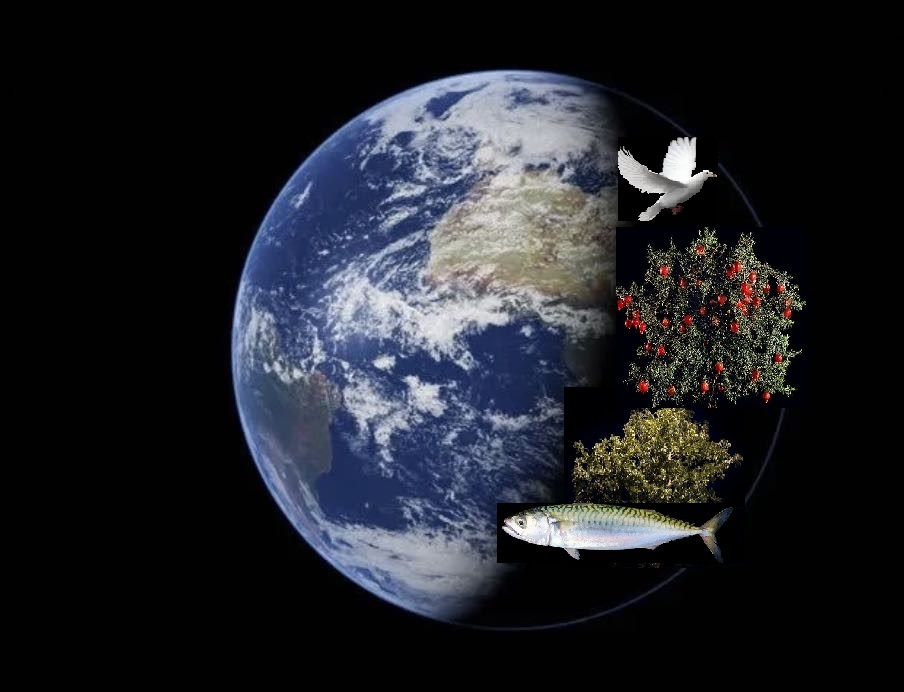
\includegraphics[width=\textwidth]{ZongJie/bibleAdult/fig/2ndday}  
  
\end{center}
     \end{subfigure}
\end{figure}


\begin{figure}
 \centering
\begin{subfigure}[b]{0.3\textwidth}
         \centering
    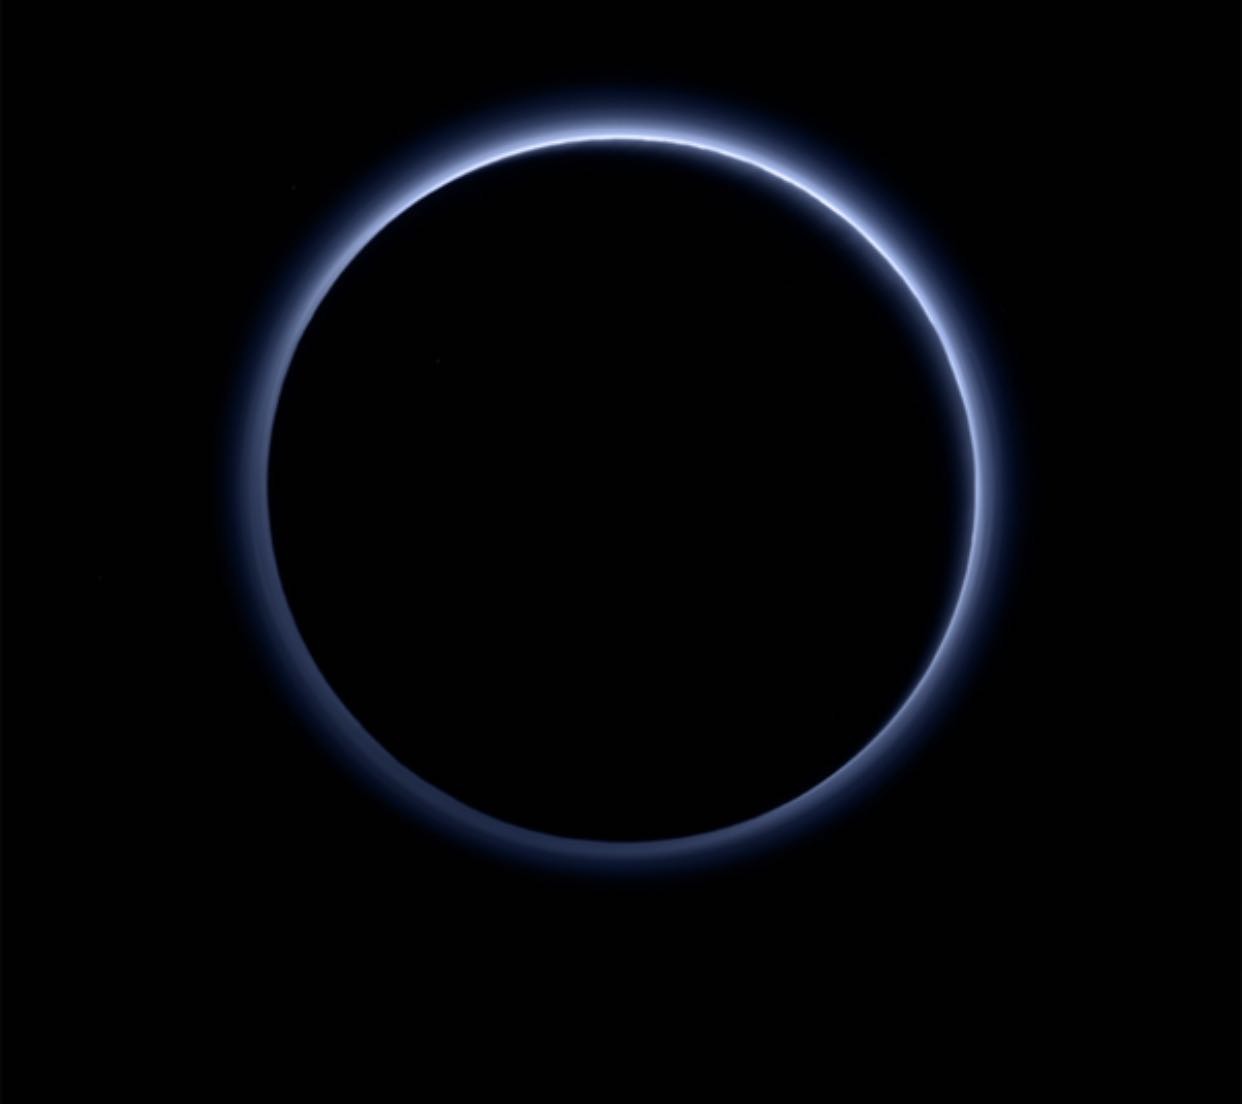
\includegraphics[scale=0.1, ]{ZongJie/bibleAdult/fig/beginning}
     %    \caption{creation of sun,moon and stars}
     %    \label{fig:y equals x}
     \end{subfigure}
     \hfill
     \begin{subfigure}[b]{0.3\textwidth}
         \centering
         
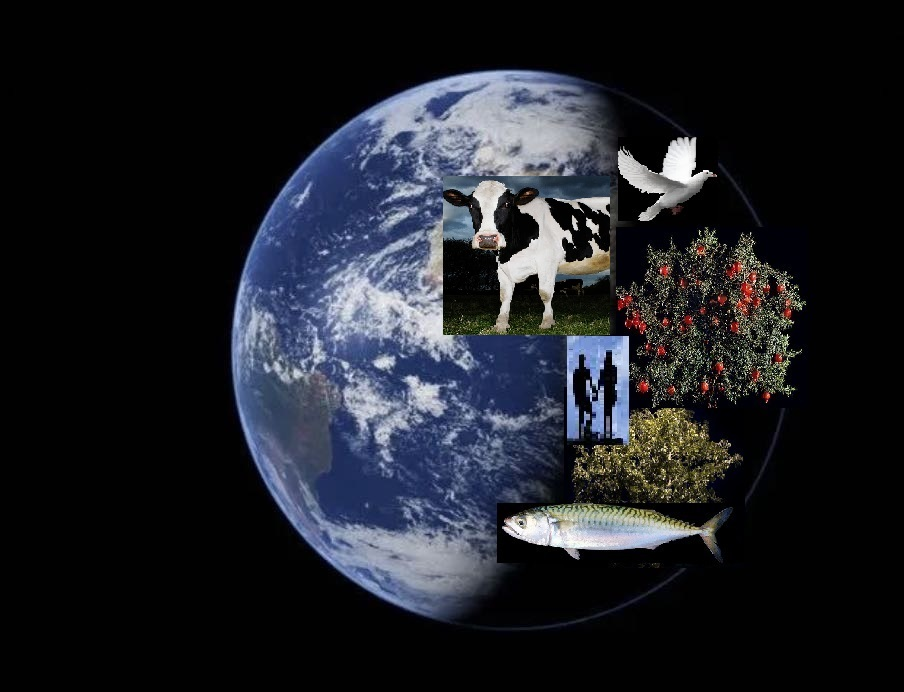
\includegraphics[width=\textwidth]{ZongJie/bibleAdult/fig/6day2}
     \end{subfigure}
     \hfill
     \begin{subfigure}[b]{0.3\textwidth}
         \centering
         
  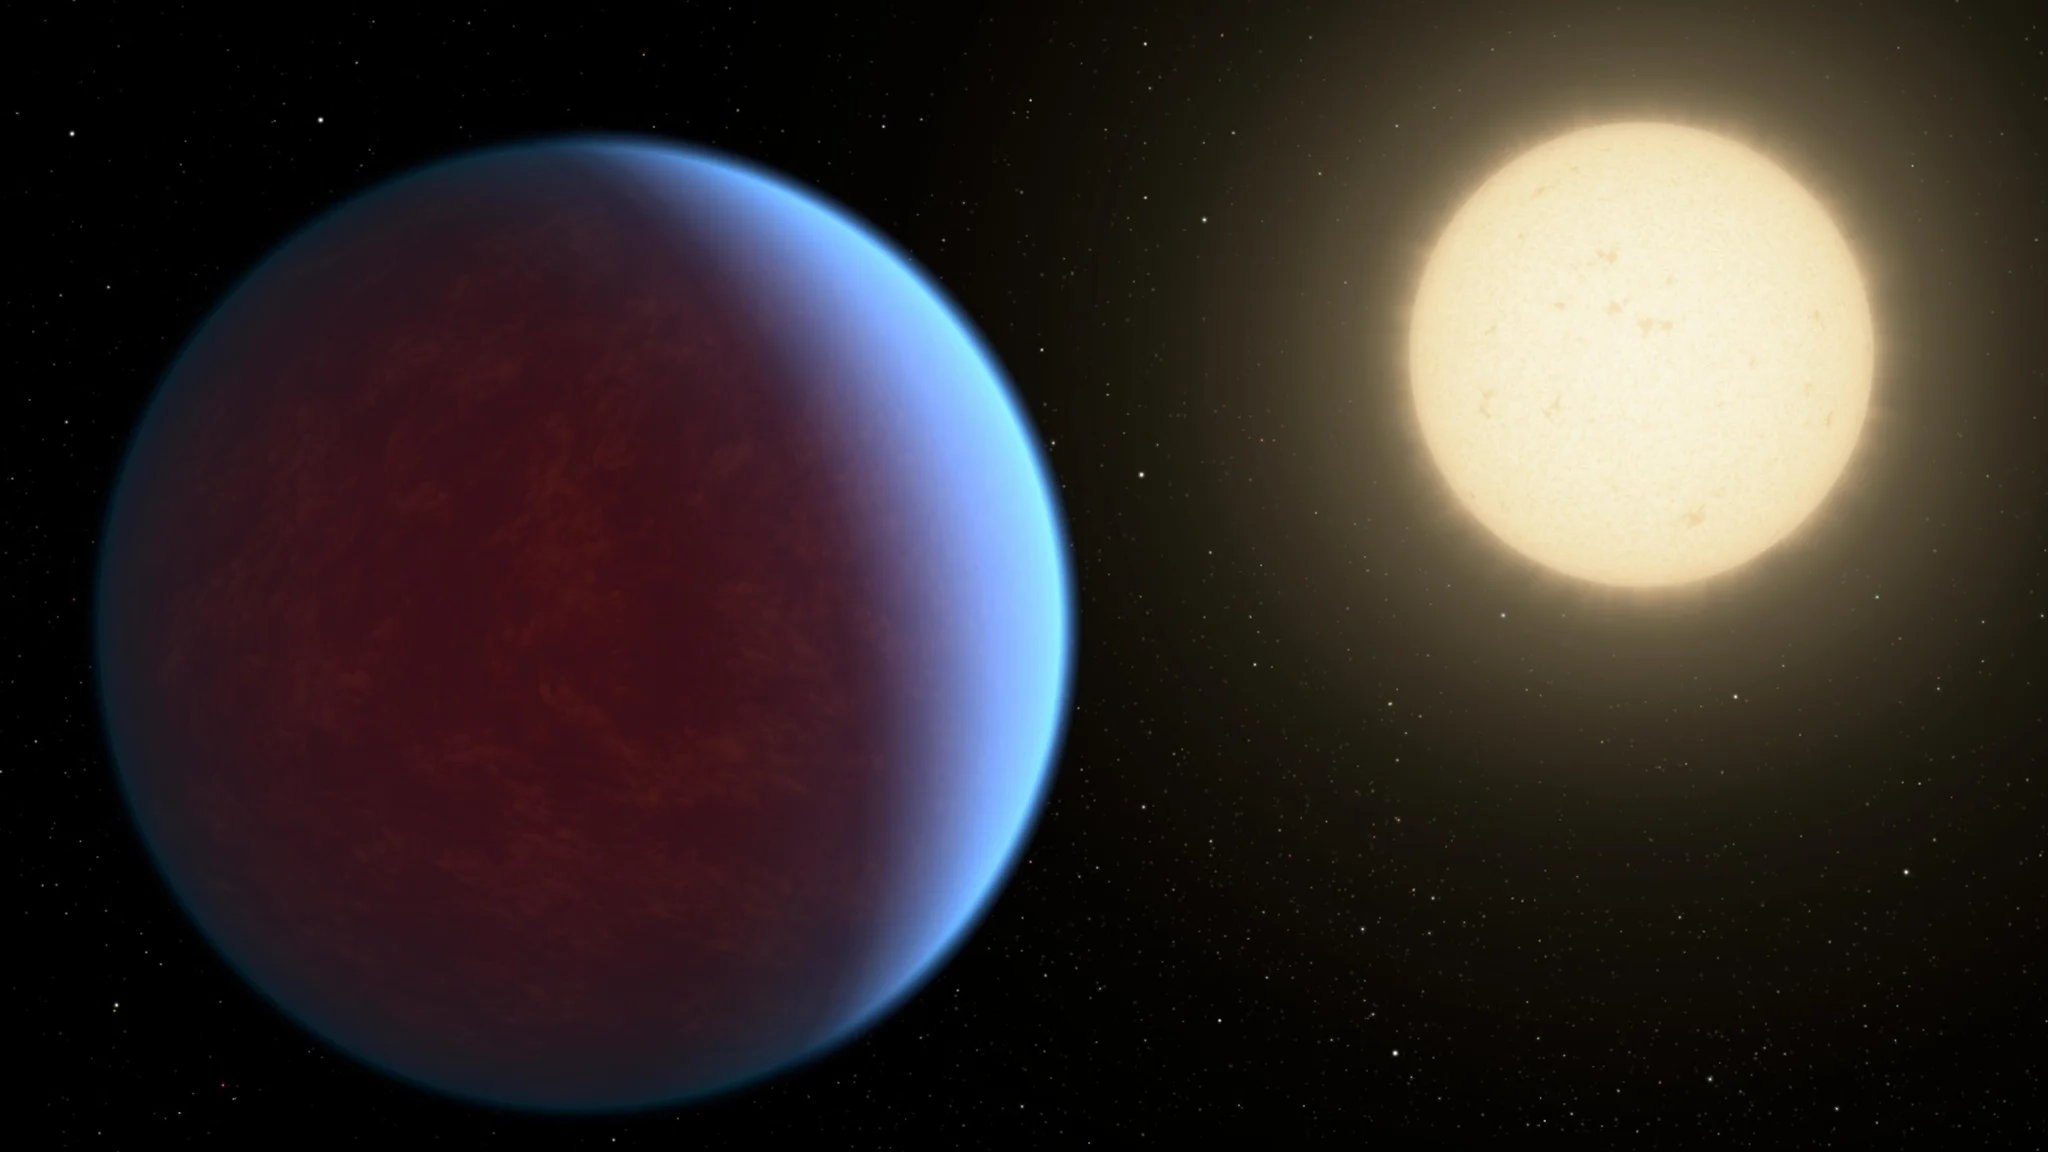
\includegraphics[scale=0.36, ]{ZongJie/bibleAdult/fig/day1}
     \end{subfigure}
  
\end{figure}


\iffalse
\begin{figure}
\centering
     \begin{subfigure}[b]{0.3\textwidth}
         \centering
         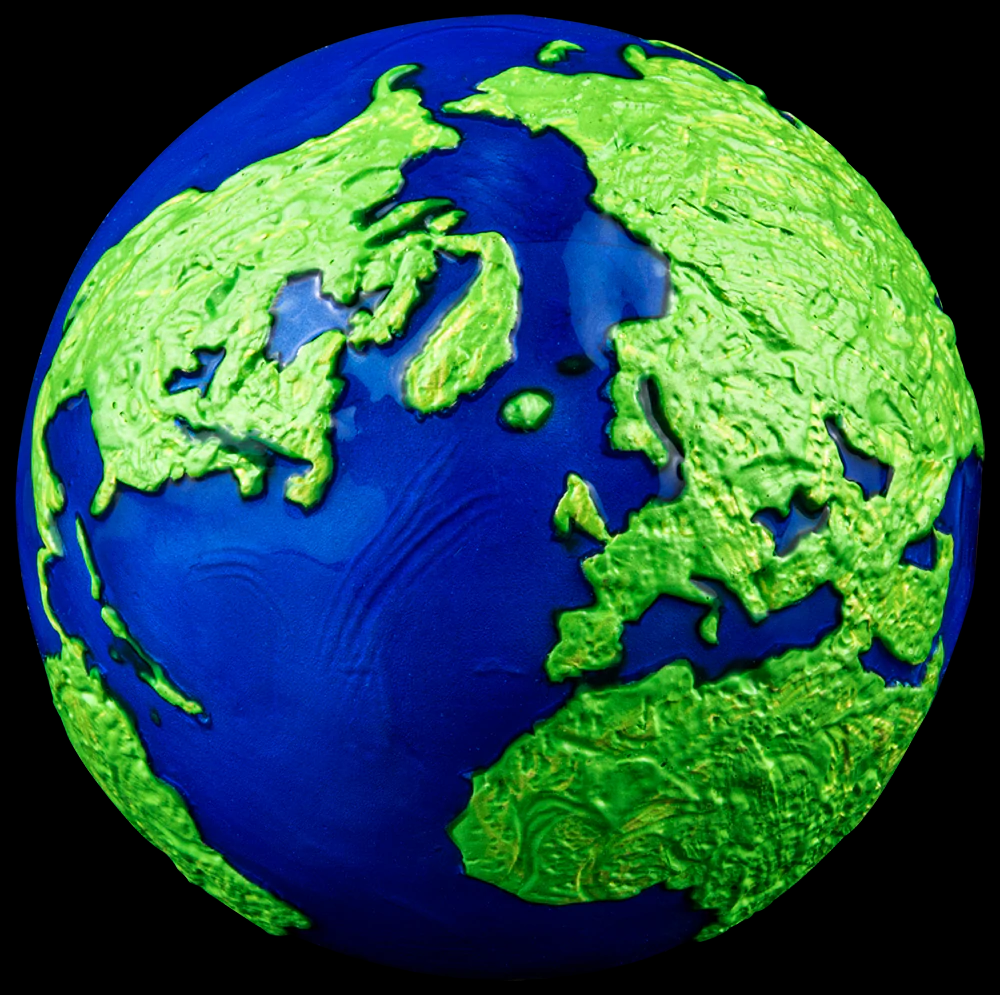
\includegraphics[scale=0.613, ]{ZongJie/bibleAdult/fig/day3}
\caption{day 3: the land and the sea}
     \end{subfigure}
     \hfill
     \begin{subfigure}[b]{0.3\textwidth}
         \centering
         \includegraphics[scale=0.613, ]{ZongJie/bibleAdult/fig/day32}
\caption{day 3: the tree and grass}
     \end{subfigure}
\end{figure}

\begin{figure*}[H]
    \begin{subfigure}[b]{0.35\textwidth}
         \centering
         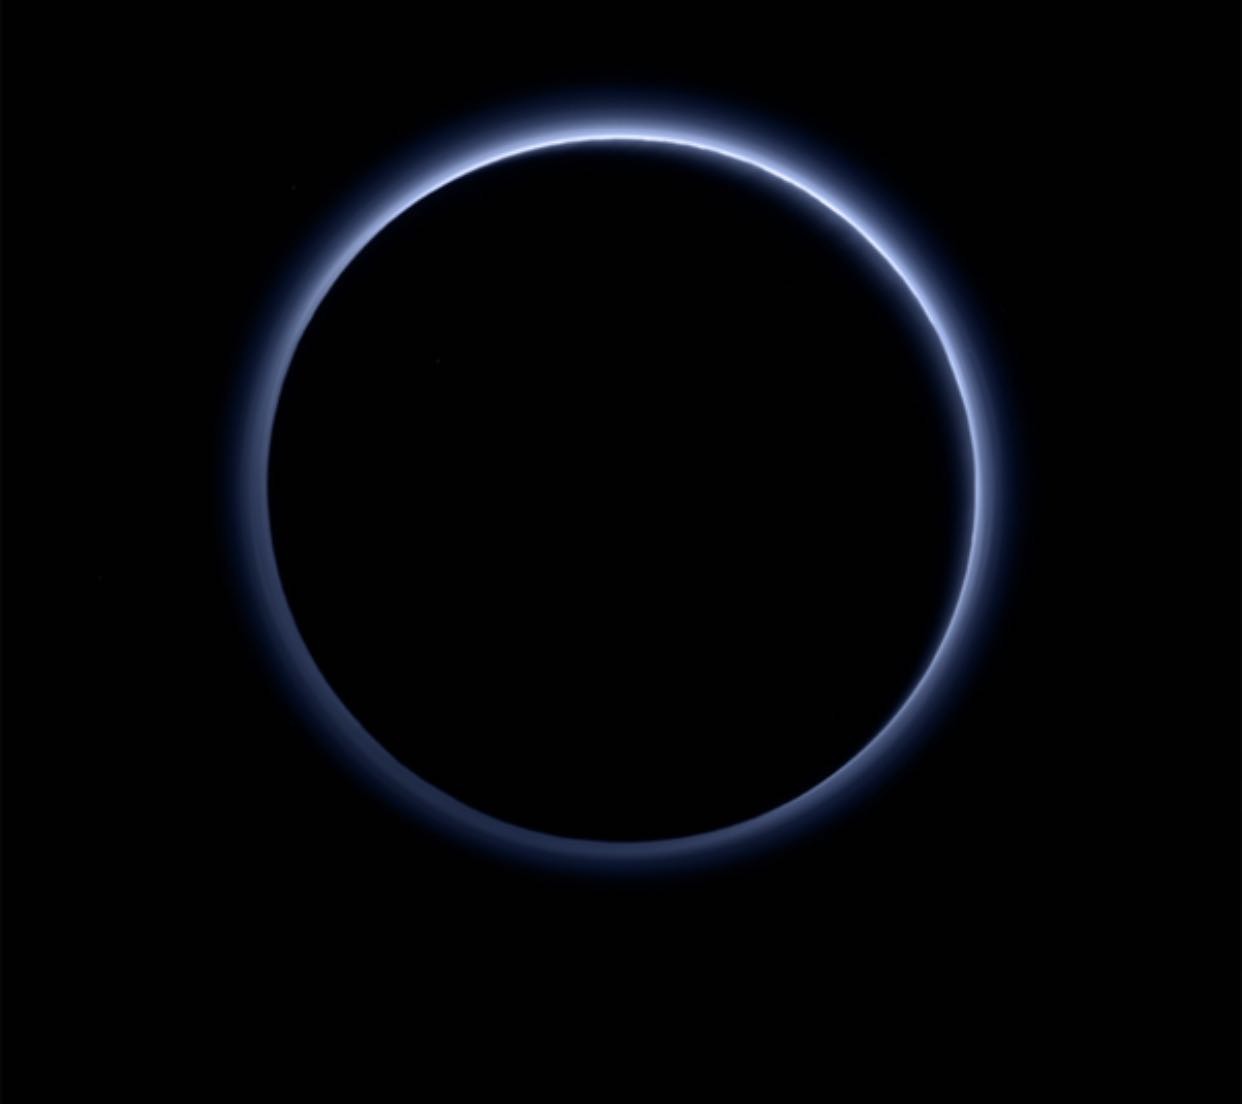
\includegraphics[height=1.86in]{ZongJie/bibleAdult/fig/beginning}
\caption{beginning}
     \end{subfigure}
  ~ 
    \centering
    \begin{subfigure}[b]{0.35\textwidth}
        \centering
        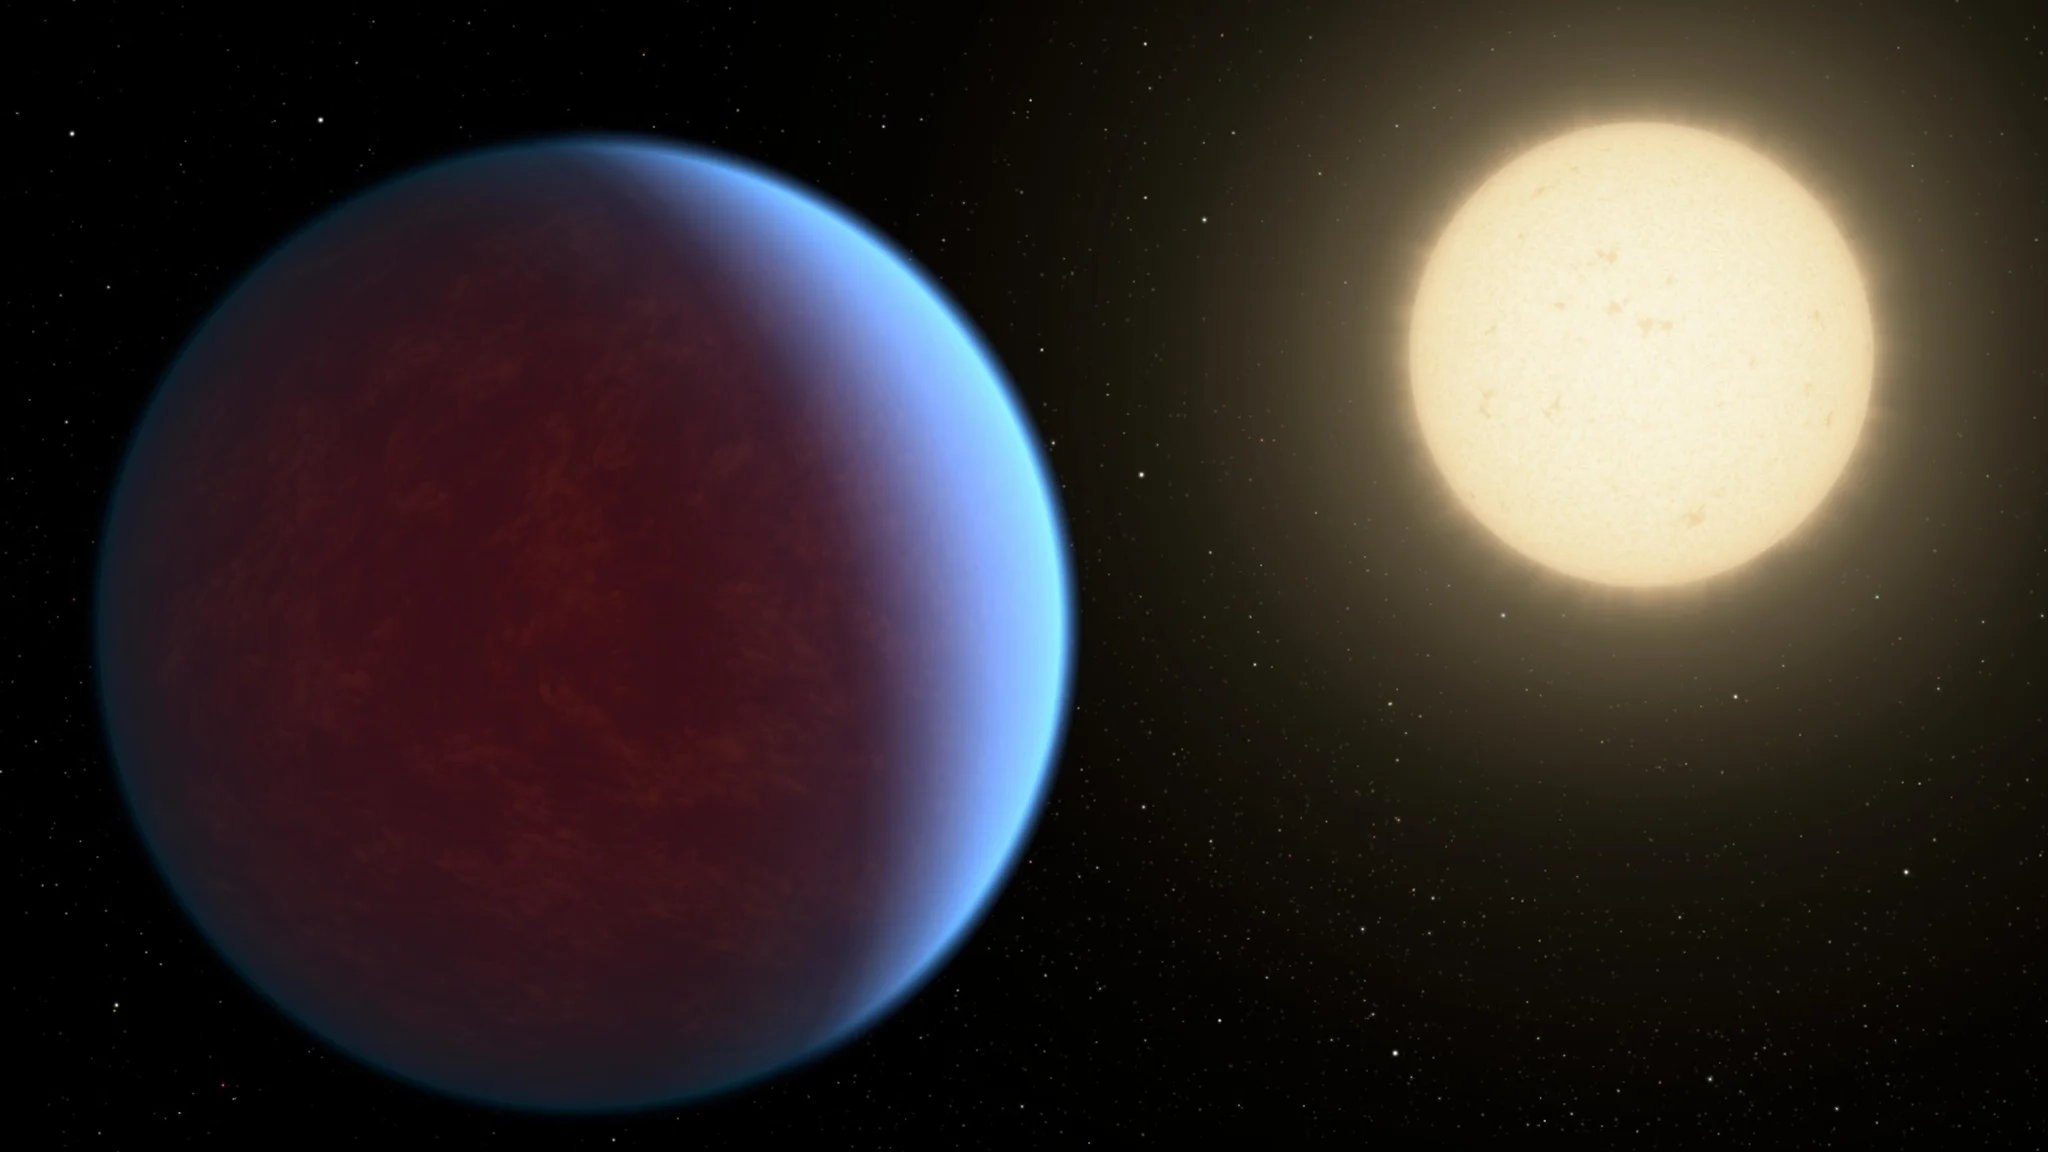
\includegraphics[height=1.86in]{ZongJie/bibleAdult/fig/day1}
        \caption{1st day: light}
    \end{subfigure}%
  ~ 
    \begin{subfigure}[b]{0.35\textwidth}
        \centering
        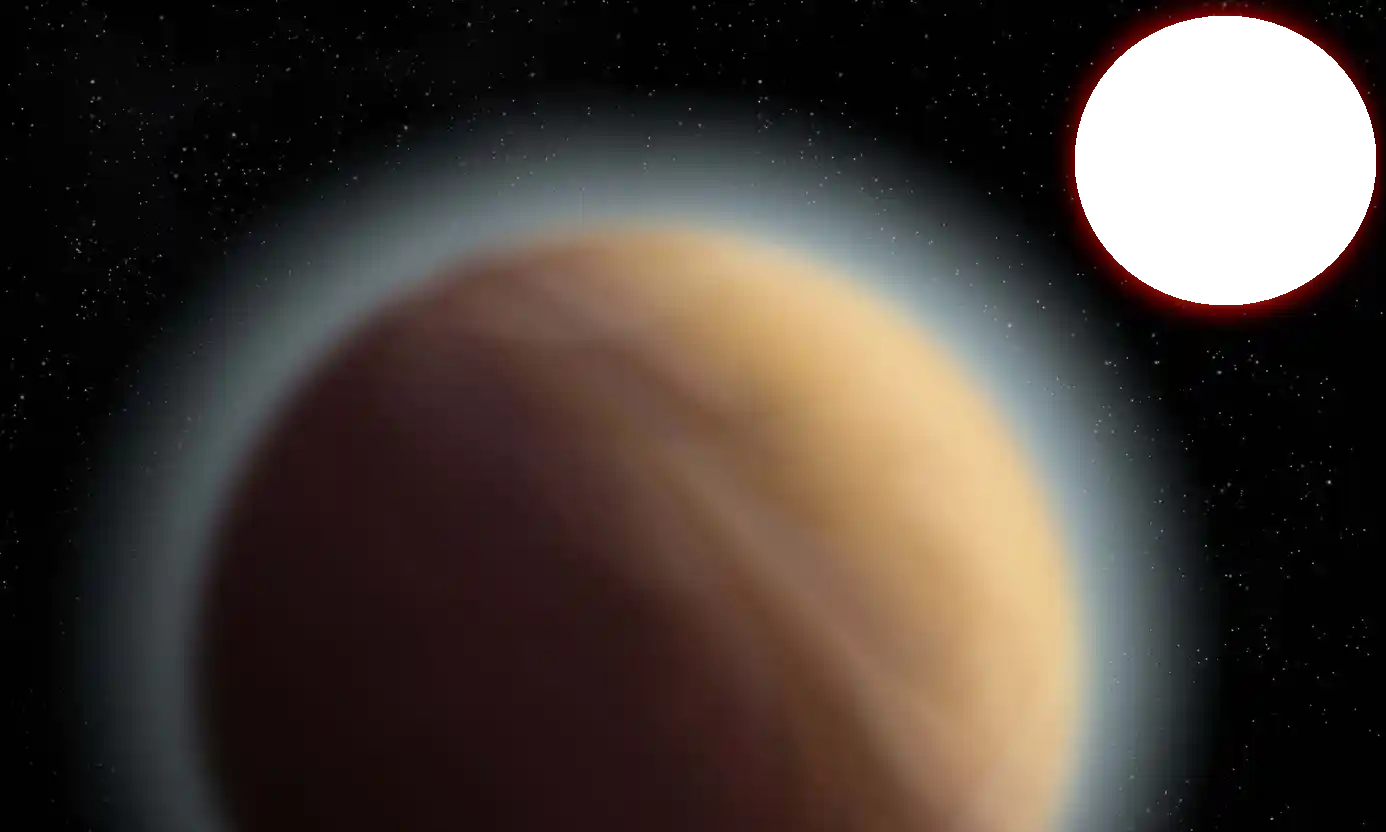
\includegraphics[height=1.86in]{ZongJie/bibleAdult/fig/day2}
      %  \caption{Lorem ipsum, lorem ipsum,Lorem ipsum, lorem ipsum,Lorem ipsum}
    \end{subfigure}
\end{figure*}

\begin{figure*}[H]
    \begin{subfigure}[b]{0.5\textwidth}
         \centering
         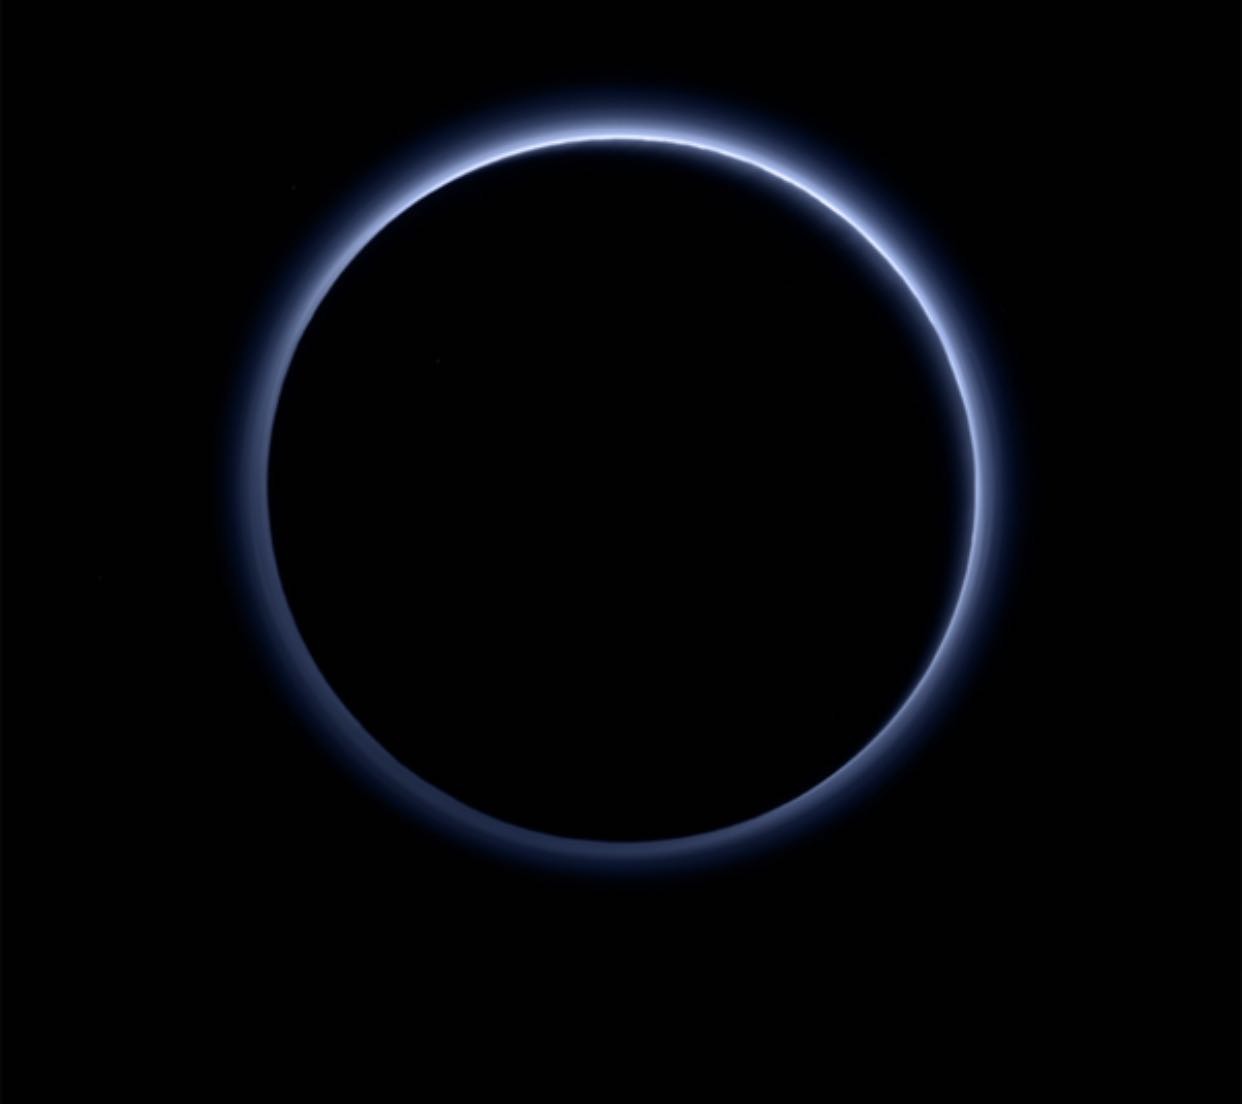
\includegraphics[height=1.86in]{ZongJie/bibleAdult/fig/beginning}
\caption{beginning}
     \end{subfigure}
    ~ 
    \begin{subfigure}[b]{0.5\textwidth}
        \centering
        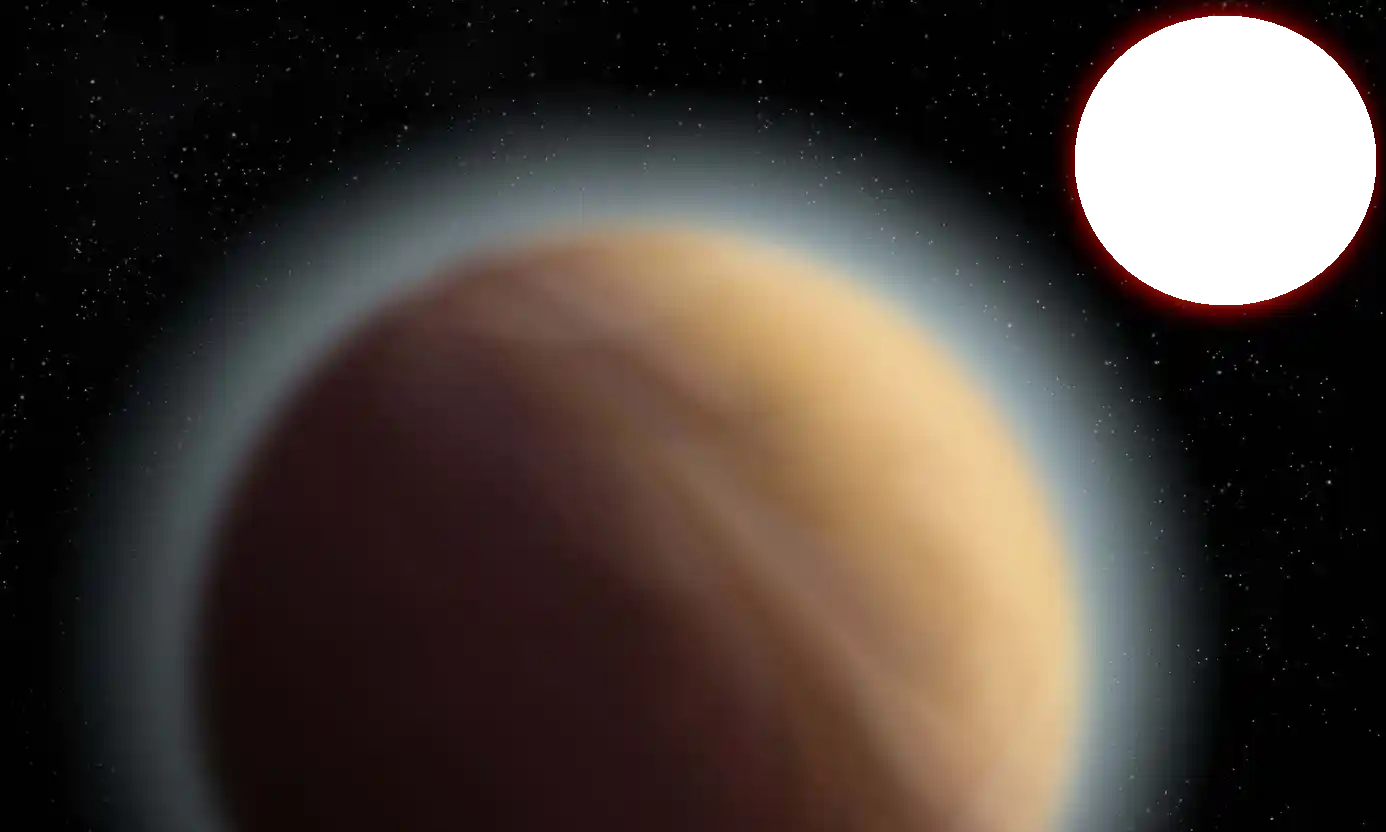
\includegraphics[height=1.86in]{ZongJie/bibleAdult/fig/day2}
      %  \caption{Lorem ipsum, lorem ipsum,Lorem ipsum, lorem ipsum,Lorem ipsum}
    \end{subfigure}
  %  \caption{Caption place holder}
\end{figure*}


https://www.shutterstock.com/image-photo/earth-space-telescope-1261029271
\fi

